%************************************************
\chapter{Introduction}\label{ch:introduction}
%************************************************
\section{Survey}
\label{sec:survey}
\acp{DNA}  and \acp{RNA} are macromolecules in the nucleus of eukaryotic cells that allow storing information with the help of nucleotides. Nucleotides consist of a five-carbon sugar, a phosphate group, and a nucleobase. There are four nucleotides in the \ac{DNA}, distinguished by their nucleobases: A for Adenine, T for Thymine, G for Guanine, and C for Cytosine. Similar to \ac{DNA}, we also find four different nucleotides in \ac{RNA}, also distinguished by their nucleobases with only one exception; the Uracil (U), which replaces Thymine in \ac{DNA}. Even though the basis blocks constituting the \ac{DNA} were known for many years, in 1953, James Watson and Francis Crick \cite{watson1953molecular} succeeded in putting them together and suggested a reasonable \ac{DNA} structure. Their work revealed for the first time that the structure of \ac{DNA} molecules has helical chains, each coiled round the same axis where the chain consists of phosphate dieter groups. The two chains are held together by the purines and pyrimidine bases; they are joined together in pairs, a single base from the other chain bonded to a single base from one chain. For the biding to occur, one of the pairs must be Adenine and Thymine or Guanine and Cytosine. A \ac{DNA} molecule structure is depicted on the right side of the page. In contrast to \ac{DNA}, \acp{RNA} are mostly single-stranded, and the complementary pairings formed in the structure are A-U, G-U and G-C.  
\graffito{\includegraphics[width=1\linewidth]{../res/images/dna.png}
	Helical representation of \ac{DNA} structures \cite{watson1953molecular}.}

Watson and Crick's elucidation of \ac{DNA} structure has motivated many other scientists to investigate further the structural implications of molecules in functions such as replication and gave rise to modern molecular biology. Later in the same year, Crick formulated the central dogma of molecular biology that describes the flow of information from \ac{DNA} to \ac{mRNA} through transcription and from mRNAs to proteins through translation  \cite{crick1970central}. Since this information flow was proposed, more works have been done to investigate each step. 

But not all \acp{RNA} are translated into proteins; in other terms, not all \acp{RNA} are \acp{mRNA}. There are mainly two \ac{RNA} groups: \acp{cRNA} that are translated into proteins, and non-coding \acp{RNA} that are not translated into proteins. During the transcription and translation steps in the information flow, some vital functions are performed by \acp{ncRNA} such as \ac{rRNA} and \ac{tRNA}. The tertiary structure of a \ac{tRNA} is shown on the left side of the page.
\graffito{\includegraphics[width=1\linewidth]{../res/images/tertiary.png}
	The tertiary structure of \ac{tRNA}. The CCA-tail is in yellow, the acceptor stem in purple, the variable loop in orange, D-arm in red, the anticodon arm in blue with anticodon in black, and T-arm in green (Taken from Wikipedia)}
The study of such \acp{RNA} revealed that \acp{rRNA}, rather than ribosomal proteins, catalyze the synthesis of proteins (i.e. the polymerization of amino acids), distinguish between correct and incorrect codon-anticodon pairs and prevent the premature hydrolysis of peptidyl-tRNAs \cite{moore2011roles, breaker2006rna}. Apart from being central to the protein machinery, \acp{ncRNA} regulate various biological functions in transcriptional interference, telomere maintenance, epigenetic changes, imprinting, post-transcriptional, translational control, structural organization, cell differentiation and development \cite{fatica2014long,santosh2015non}. We are interested in this work in the structures of \acp{ncRNA}.

The function of \acp{ncRNA} is largely determined by their high-dimensional structure \cite{cech2014noncoding}. For instance, we can analyze the catalytic function of ribozymes in terms of basic structural motifs, e.g. hammerhead or hairpin structures \cite{doherty2001ribozyme}. Other \acp{RNA}, like riboswitches, involve changes between alternative structures  \cite{vitreschak04_ribos}. Understanding the relation sequence and structure is a central challenge in molecular biology. In the last $20$ years, many different methods for determining the \ac{RNA} structures of molecules have emerged: from experimental lab methods to computational approaches. For experimental lab methods, X-ray crystallography and the \ac{NMR} are the most accurate approaches to offer structural information at a single base-pair resolution. Both experimental methods are often characterized by high experimental cost and low throughput. In addition to those limitations, \ac{RNA} molecules are volatile and difficult to crystallize.

Despite the development of more sophisticated techniques to infer the state of nucleotides in \ac{RNA} molecules using enzymatic \cite{kertesz2010genome, underwood2010fragseq} or chemical probes \cite{tijerina2007dms, wilkinson2006selective} coupled with next-generation sequencing \cite{bevilacqua2016genome, tian2016rna}, most of them can only capture \ac{RNA} structures \textit{in vitro} which mostly differ from the \textit{in vivo} structure conformations. Experimentally, only a tiny fraction of known \acp{ncRNA} has been determined \cite{rnacentral2017rnacentral}. Because measuring the structure of \acp{RNA} experimentally is very difficult and expensive, computational approaches play a central role in the analysis of natural \acp{RNA} \cite{seetin2012rna, fallmann2017recent}, and are an essential alternative to experimental approaches. 

Given the \ac{ncRNA} sequence of bases (primary structure), RNAs fold into secondary structures, such as stem loops and pseudoknots, before folding into higher level (tertiary and quaternary) structures \cite{brion1997hierarchy,tinoco1999rna}. This separation of time scales justifies focusing on the secondary structure prediction; evidence suggests that the \ac{RNA}'s secondary structures largely determine the resulting high-level structures \cite{tinoco1999rna}. 

This thesis focuses on computational methods addressing \ac{RNA} molecules' folding and inverse folding at the secondary level. This introductory chapter presents a brief overview of the non-coding \ac{RNA} concepts. The overview concepts contain biological and biochemical structure definitions of the non-coding \acp{RNA}. It also gives an overview of different techniques used to identify new \acp{ncRNA} and some applications. It concludes by providing the bioinformatic definitions of \ac{RNA} secondary structure that constitute the basis and understanding of computational methods and the results presented in this thesis.

\section{Characteristics and biological functions of ncRNA} 
\label{sec:biological_function}
In the previous section, we introduced the classical view of information flow in microbiology. Two important \acp{ncRNA} involved in the protein machinery have been highlighted (\ac{tRNA} and \ac{rRNA}). In this section, we provide some of the main characteristics of \acp{ncRNA}, and we emphasize how those characteristics often play an essential role in realizing their functions. 

What motivates the computational studies of \acp{ncRNA} is often the importance of the biological function they play. Consequently, the \acp{ncRNA} can be classified based on their biological functions. Although many recent transcriptomic and bioinformatic studies suggested thousands of \acp{ncRNA} with their functional importances, the total number of \acp{ncRNA} encoded in the human genome still remains unknown \cite{santosh2015non}. More recently, newly identified \acp{ncRNA} have not been validated by their function; it could be possible that most of them are non-functional. Some  evolutionary experiments \textit{in vitro} have shown that \ac{RNA} molecules can catalyze various chemical reactions relevant to biological processes such as \ac{RNA} replication, nucleotide synthesis, thymidylate synthesis, lipid synthesis, and sugar metabolism \cite{robertson1990selection,ellington2009evolutionary}. 
Another characteristic of \acp{ncRNA} is their lengths formed post-transcriptionally. We often distinguish two main \ac{ncRNA} classes of critical biological functions: the \acp{sncRNA} (with length $<30nt$) and the \acp{lncRNA} (with length $>200nt$). The length limit is often because of the practical considerations, including separating \acp{RNA} in standard experimental protocols. The length of \acp{ncRNA} is also taken into account in computational studies, and it will be used throughout our work to distinguish \ac{RNA} sequences and structures in the different datasets considered.

The function of \acp{lncRNA} includes a role in higher-order chromosomal dynamics, telomere biology, and subcellular structural organization \cite{bergmann2014long,cusanelli2014telomeric}. Some \acp{lncRNA} play key regulatory and functional roles in the gene expression program of the cell. One of the vital functions is to act as ribozymes. Examples of naturally occurring ribozymes include group I and group II introns---RNase P and the hammerhead. The group, I and group II introns are usually $200-600$nt long, catalyzing \ac{RNA} splicing \cite{gilbert_origin_1986}. Many \acp{sncRNA} also contribute to the realization of similar biological functions. For example, small interfering \acp{RNA} contribute to gene regulation, transposon control and vital defence. \acp{miRNA} participate in the post-transcriptional gene regulation, \acp{miRNA}, \acp{piRNA}) and \acp{PAR} contribute to the gene regulation. More recently,  many discoveries revealed several \acp{ncRNA} implicated in cancer growth and MCL-1 expression regulation \cite{wang2021circpvt1, santosh2015non}. Those examples include \acp{ncRNA} from different classes, \acp{miRNA}, \acp{snoRNA} and T-UCR, all associated with a specific disease \cite{santosh2015non,esteller2011non}. 

There are also other classes of \acp{ncRNA} such as aptamers and riboswitches that have also been observed in nature. Aptamers are \acp{ncRNA} that can bind to other specified targets, whose nature is highly diverse. They range from small molecules to larger molecules. In some contexts, aptamers are termed riboswitches; for example, when their function is to sense the presence of an associated metabolite to cause a specific cis-reaction and/or cis-regulation of subordinated functional pathways \cite{winkler2003genetic}. 

In sum, lnc/snc-RNAs contribute to the realization of various biological functions, and they are mostly distinguishable based on their length and functions. But, their functions allow us to distinguish them better. In the next section, we provide some of the recent advancements in the techniques used to identify functional \acp{ncRNA}.

\section{Recent advancements in determining ncRNA functions}
\label{sec:advancements}
Most of the previously mentioned functions of \acp{ncRNA} are identified using gene targeting techniques, a well-known set of techniques used to investigate protein functions \cite{sauvageau2013multiple}. In addition, experimental approaches are used to define \ac{ncRNA} functions. With the recent advancements in genome engineering, a method such as \ac{CRISPR} has been employed to tag \acp{lncRNA}, allowing to capture specific \ac{RNA}-protein complexes assembled \textit{in vivo}. This section aims at providing an overview of different techniques used to determine \ac{ncRNA} functions.

The  \ac{CRISPR} \cite{barrangou2007crispr} was described by Barrangou and his collaborators in 2007 as a distinctive genome feature of most bacteria and archaea and thought to be involved in resistance to bacteriophages. It is an adaptive defence system against viruses and plasmid intrusions. When a successful defence takes place, the system updates information about the intruder's genetic material. This update will then allow the system's host to identify its enemy, making it robust and durable in the future. The information about the intruder's genetic material is stored in short repeating stretches of \ac{RNA}, which can, in the case of a new intrusion, be incorporated into a carrier protein(CAS). The capacities of the   \ac{CRISPR}/CAS9 of selectively destroying foreign \ac{DNA}/\ac{RNA} and editing the genome was identified by Li et al. \cite{li2016harnessing}, and it was turned into methods allowing to alter and edit single genes within genomes selectively. The same technology is also successfully applied to animal cell lines \cite{hwang2013efficient, jinek2013rna, wang2013one} and industrial plants \cite{svitashev2015targeted,li2015cas9}. 

Another method of \ac{SELEX} \cite{tuerk1990systematic} introduced by Tuerk in the early 1990s offers the possibility of enriching stretches of \ac{RNA} that can bind a certain target. The method relies on mechanisms usually ascribed to the process of evolution, that is, variation, selection, and replication. A pool of \acp{RNA} that are entirely randomized at specific positions is subjected to selection for binding, in this case to GP43 on nitrocellulose filters. The selected \acp{RNA} are amplified as double-stranded \ac{DNA} competent for subsequent \textit{in vitro} transcription. This newly transcribed \ac{RNA} is enriched for better binding sequences and is then subjected to selection to begin the next cycle. Multiple rounds of enrichment result in the exponential increase of the best binding ligands until they dominate the population of sequences. \ac{SELEX} has given rise to numerous synthetic aptamers with different targets in its application. They have been subject to a further extension towards inclusion into regulative \ac{RNA} entities.

More recently, increased types of \acp{ncRNA} have been detected and identified by the development of next-generation sequencing \cite{wang2009rna}, which can be roughly divided into the process sections of sample preprocessing, library preparation, sequencing, and bioinformatics. 

The functions of many \acp{ncRNA} are dependent on their high-level structures, which often depend on lower-levels sequence and secondary structures. Knowing the structure of an \ac{ncRNA} plays a vital role in probing its function. For example, Peter Flor and his collaborators used structure information to interpret experiments related to the mechanism of \ac{RNA} function \cite{flor1989conserved}. Or, Yoon et al. suggested new experiments based on RNA secondary structure in yeast to probe RNA functions \cite{kim2007staufen1}. Therefore, understanding even the secondary structure alone can assist both of these examples. In the following section, we provide a biochemical definition of the elementary building blocks of \acp{ncRNA}, which are the nucleotides A, U, G and C. In addition, we will provide an overview of the different nucleotide interactions involved during the formation of their secondary structures. 

\section{Biochemistry of RNA molecules}
\label{sec:rna_biochemical}

\graffito{
	\hspace*{-1cm}
	\scalebox{0.95}{
		
		\chemname[1cm]{\chemfig{
				-[,1.202,,,line width=3.5pt, shorten <=-.05pt, shorten >=-.05pt](-[:-90,,,,line width=1.5pt, shorten >=.5pt]OH)% 2
				>[:44.6,0.521](-[:90, 3.3]{\textcolor{blue}{Nucleobase}})
				-[:167]\chembelow[35pt]{O}{Ribose}
				-[:193,0.998]
				(
				-[:90](-[,0.1,,,draw=none]\chemabove[1ex]{}{\textcolor{gray}{5'}})
				-[::90,1.,,,red](-[::0,,,,red]\color{red}{P}(-[2,,,,red]\color{red}{O^{-}})(-[4,1.3,,,red]\color{red}{O^{-}})(=[6,,,,red]\chembelow{\color{red}{O}}{\textcolor{red}{Phosphate}}))
				)
				(
				<[:315.6,0.522](-[:-90,,,,line width=1.5pt, shorten >=.5pt]OH)(-[::-150,0.4,,,draw=none]\chembelow[1ex]{}{\textcolor{gray}{3'}})
				)
		}	}{Structure of an \ac{RNA} nucleotide}
	}
	%	\vspace*{6cm}\\
	%	\includegraphics[width=1\linewidth]{../res/images/mfe.png}
	%	An example of secondary structure with a \ac{MFE} of $8.5$kcal.$mol^{-1}$ (Produced using \texttt{RNAfold} from the \texttt{ViennaRNA} package)
}
So far, we have provided a biological motivation for studying \ac{ncRNA} as an independent entity. The discovery of new \acp{ncRNA} functions has emerged through intensive experimental studies and with recent advanced techniques in next-generation sequencing. Several examples demonstrated the importance of the \ac{ncRNA} structures in the probing process of new functions. The process in which \ac{RNA} sequences are mapped to their corresponding structures is called \ac{RNA} folding. In nature, this process is thought to be hierarchical \cite{brion1997hierarchy,tinoco1999rna}. Nucleotides form a chain given their sequence of bases (primary structure); \acp{RNA} fold into secondary structures, such as stem-loops and helices, before folding into higher-level (tertiary and quaternary) structures. Our work is restricted here to the secondary level of an \ac{RNA} structure, i.e., the set of canonical pairs. This section provides a biochemical definition of different nucleotides and base-pair interactions involved in the secondary structure folding of \ac{RNA} molecules. 

%\reversemarginpar

Chemically, each nucleotide in \ac{RNA} molecules consists of a phosphate residue, a pentose sugar and a nucleobase. The typical chemical structure of a nucleotide is depicted on the right side of the page. \autoref{fig:nucleotide} illustrates the chemical structure of each of the four different nucleobases found in \ac{RNA} (A, C, G and U). A nucleotide is a nucleoside which has a (mono, di, trip) phosphate residue bound to its 5'-carbon atom. By convention, the carbon atoms of the pentose sugar in nucleotides are numbered with \textit{primes}.

\begin{figure}[t!]
	\begin{minipage}[b]{.5\linewidth}
		\centering
		\subfloat[Adenosine 5'􏱈-monophosphate]{
			\label{fig:adenine}{
				\scalebox{0.9}{
					\chemfig{
						-[,1.202,,,line width=3.5pt](-[:-90,,,,line width=1.5pt]OH)% 2
						>[:44.6,0.521](-[:90] \color{blue}{N}*5(-[,,,,blue]*6(-[,,,,blue]\color{blue}{N}=[,,,,blue]-[,,,,blue]\color{blue}{N}=[,,,,blue](-[:90,,,,blue]\color{blue}{NH_2})-[,,,,blue]-[,,,,blue])=[,,,,blue]-[,,,,blue]\color{blue}{N}=[,,,,blue]-[,,,,blue]))
						-[:167]O
						-[:193,0.998]
						(
						-[:90](-[,0.1,,,draw=none]\chemabove[1ex]{}{\textcolor{gray}{5'}})
						-[::90]O(-[::0]P(-[2]O^{-})(-[4]O^{-})(=[6]O))
						)
						(
						<[:315.6,0.522](-[:-90,,,,line width=0.5pt]OH)(-[::-150,0.4,,,draw=none]\chembelow[1ex]{}{\textcolor{gray}{3'}})
						)
					}	
				}	
		}}\hfill
	\end{minipage}
	\begin{minipage}[b]{.5\linewidth}
		\centering		
		\subfloat[Uridine 5'-monophosphate]{
			\label{fig:uracil}{
				\scalebox{0.9}{\chemfig{
						-[,1.202,,,line width=3.5pt, shorten <=-.05pt, shorten >=-.05pt](-[:-90,,,,line width=1.5pt, shorten >=.5pt]OH)% 2
						>[:44.6,0.521](-[:90] \color{blue}{N}*6(-[,,,,blue](=[,,,,blue]\color{blue}{O})-[,,,,blue]\color{blue}{NH}-[,,,,blue](=[,,,,blue]\color{blue}{O})-[,,,,blue]=[,,,,blue]-[,,,,blue]))
						-[:167]O
						-[:193,0.998]
						(
						-[:90](-[,0.1,,,draw=none]\chemabove[1ex]{}{\textcolor{gray}{5'}})
						-[::90]O(-[::0]P(-[2]O^{-})(-[4]O^{-})(=[6]O))
						)
						(
						<[:315.6,0.522](-[:-90,,,,line width=1.5pt, shorten >=.5pt]OH)(-[::-150,0.4,,,draw=none]\chembelow[1ex]{}{\textcolor{gray}{3'}})
						)
				}}
		}}
	\end{minipage}
	
	\begin{minipage}[b]{.5\linewidth}
		\centering
		\subfloat[Cytidine 5'􏱈-monophosphate]{
			\label{fig:cytosine}{
				\scalebox{0.9}{	\chemfig{
						-[,1.202,,,line width=3.5pt, shorten <=-.05pt, shorten >=-.05pt](-[:-90,,,,line width=1.5pt, shorten >=.5pt]OH)% 2
						>[:44.6,0.521](-[:90]\color{blue}{N}*6(-[,,,,blue](=[,,,,blue]\color{blue}{O})-[,,,,blue]\color{blue}{N}=[,,,,blue](-[,,,,blue]\color{blue}{NH_2})-[,,,,blue]=[,,,,blue]-[,,,,blue]))
						-[:167]O
						-[:193,0.998]
						(
						-[:90](-[,0.1,,,draw=none]\chemabove[1ex]{}{\textcolor{gray}{5'}})
						-[::90]O(-[::0]P(-[2]O^{-})(-[4]O^{-})(=[6]O))
						)
						(
						<[:315.6,0.522](-[:-90,,,,line width=1.5pt, shorten >=.5pt]OH)(-[::-150,0.4,,,draw=none]\chembelow[1ex]{}{\textcolor{gray}{3'}})
						)
					}
				}
		}}
	\end{minipage}%
	\begin{minipage}[b]{.5\linewidth}
		\centering 
		\subfloat[Guanosine 5'􏱈-monophosphate]{
			\label{fig:guanine}{
				\scalebox{0.9}{	
					\chemfig{
						-[,1.202,,,line width=3.5pt, shorten <=-.05pt, shorten >=-.05pt](-[:-90,,,,line width=1.5pt, shorten >=.5pt]OH)% 2
						>[:44.6,0.521](-[:90] \color{blue}{N}*5(-[,,,,blue]*6(-[,,,,blue]\color{blue}{N}=[,,,,blue](-[,,,,blue]\color{blue}{NH_2})-[,,,,blue]\color{blue}{NH}=[,,,,blue](=[:90,,,,blue]\color{blue}{O})-[,,,,blue]-[,,,,blue])=[,,,,blue]-[,,,,blue]\color{blue}{N}=[,,,,blue]-[,,,,blue]))
						-[:167]O
						-[:193,0.998]
						(
						-[:90](-[,0.1,,,draw=none]\chemabove[1ex]{}{\textcolor{gray}{5'}})
						-[::90]O(-[::0]P(-[2]O^{-})(-[4]O^{-})(=[6]O))
						)
						(
						<[:315.6,0.522](-[:-90,,,,line width=1.5pt, shorten >=.5pt]OH)(-[::-150,0.4,,,draw=none]\chembelow[1ex]{}{\textcolor{gray}{3'}})
						)
					}
				}
				
		}}
	\end{minipage}%
	
	
	\caption{\textbf{\ac{RNA} nucleotides.} Adenine and guanine belongs into the chemical class of purine molecules and the uracil and thymine in the class of pyrimidines}\label{fig:nucleotide}
\end{figure}


At the lowest level, \ac{RNA} molecules are simply represented as a list of nucleobase characters. The 5'-3' phosphodiester bonds attach the different nucleotides composing the \ac{RNA} molecule between ribose to form the primary structure of \ac{RNA}. The chain direction is conventionally designed as 5' to 3' (i.e. from 5'-phosphate first sugar backbone to the 3'-hydroxyl last sugar in the sequence). 

In contrast to the \ac{RNA} primary structure, the secondary structure consists of a list of nucleobase-pairs, and the hydrogen bonds between the bases form base-pairs. Different interactions are possible between the bases depending on the structure level considered. At the secondary level, we have the Watson-Crick (or canonical) pairs \cite{seeman1976rna, rosenberg1976rna} (A-U and G-C), the Wobble (or non-canonical) (G-U) pairs that occur with reduced frequency. \autoref{fig:basepairing} shows the chemical base-pairs for the Watson-Crick and Wobble interactions. 


\begin{figure}{t!}
	%\hspace*{-4cm}
	\begin{minipage}[b]{1.0 \linewidth}
		\centering
		\subfloat[Adenine-Uracil Interaction]{
			\chemfig{
				R-[::42] N*5(
				%(-H)
				-(*6(
				-N=-N?[h1]
				=(-N([::60]-H)([::-60]-H?[h0]))-=
				))
				--N=-
				)
				*5(-[,,,,draw=none](*6(-[,,,,draw=none]-[,,,,draw=none]-[,,,,draw=none](-[,,,,draw=none]))))
				\phantom{A}-[,1.95,,,draw=none]
				-[::-60,2,,,draw=none]-[,2,,,draw=none]-[::120,,,,draw=none]
				N*6(%(-H)
				-=-(=O?[h0,,{dash pattern=on 1pt off 4pt}, {line width=1.5pt}, gray])-N(-H?[h1,,{dash pattern=on 1pt off 4pt}, {line width=1.5pt}, gray])-(=O?[h2,,{dash pattern=on 1pt off 4pt}, {line width=1.5pt}, gray])-)
				-[::180]R
			}
			
		}
	\end{minipage}
	\begin{minipage}[b]{1.0 \linewidth}
		\centering
		\subfloat[Guanine-Cytosine Interaction]{
			\chemfig{
				R-[::42]	N*5(
				%(-H)
				-(*6(
				-N=(-{NH_2})
				-N(-H?[h2])
				-(=O?[h1])-=
				))
				--N=-
				)
				*5(-[,,,,draw=none](*6(-[,,,,draw=none]-[,,,,draw=none]-[,,,,draw=none](-[,,,,draw=none]))))
				\phantom{A}-[,1.95,,,draw=none]
				-[::-60,2,,,draw=none]-[,2,,,draw=none]-[::120,,,,draw=none]
				*6()
				N*6(%(-H)
				-=-(-N([::60]-H?[h1,,{dash pattern=on 1pt off 4pt}, {line width=1.5pt}, gray])([::-60]-H))=N?[h2,,{dash pattern=on 1pt off 4pt}, {line width=1.5pt}, gray]-(=O?[h3,,{dash pattern=on 1pt off 4pt}, {line width=1.5pt}, gray])-)
				-[::180]R
			}
		}
		
	\end{minipage}
	%\vspace*{0.3cm}
	\begin{minipage}[b]{1.0\linewidth}
		\centering
		\subfloat[Guanine-Uracil Interaction]{
			\chemfig{
				R-[::42]	N*5(
				%(-H)
				-(*6(
				-N=(-{NH_2})
				-N(-H?[h2])
				-(=O?[h1])-=
				))
				--N=-
				)
				*5(-[,,,,draw=none](*6(-[,,,,draw=none]-[,,,,draw=none]-[,,,,draw=none]-[,,,,draw=none](-[,,,,draw=none]))))
				\phantom{A}-[,2.95,,,draw=none]
				-[::-60,2,,,draw=none]-[,2,,,draw=none]-[::120,,,,draw=none]
				N*6(%(-H)
				-=-(=O?[h0,,{dash pattern=on 1pt off 4pt}, {line width=1.5pt}, gray])-N(-H?[h1,,{dash pattern=on 1pt off 4pt}, {line width=1.5pt}, gray])-(=O?[h2,,{dash pattern=on 1pt off 4pt}, {line width=1.5pt}, gray])-)
				-[::180]R
			}
		}
	\end{minipage}
	
	\caption{\textbf{\ac{RNA} base-pair interactions}. (a) and (b) are commonly know as Watson-Crick base-pairs. (c) is the wobble base-pair. Hydrogen bonds are indicated as grey dashed lines. Substitution of bold hydrogen residues with ribose 5-phosphate yields the corresponding nucleotides found in \ac{RNA} molecules.}\label{fig:basepairing}
\end{figure}
%\section{Pseudoknots}

In addition to the \ac{WC} and wobble interactions, we also find crossing or pseudoknotted interactions in natural \ac{RNA} that play vital roles in realizing biological functions, e.g. ribosomal frame-shifting \cite{giedroc2000structure}, regulation of translation and splicing, or the binding of small molecules \cite{gilbert2008structure, klein2009cocrystal, spitale2009structural}. Although the pseudoknots are not considered in the computational folding tool we propose in \autoref{ch:rafft}, they are essential to evaluate the performance of the computational tool we will introduce in \autoref{ch:arnaque} for RNA design. This section also presents different pseudoknot patterns found in natural \ac{RNA} and emphasizes the one considered in our work.


Pseudoknots occur when two \ac{WC}, wobble or non-canonical interactions cross each other \cite{beyongWCpairs}. Even though pseudoknots are often considered the beginning of the interaction between the secondary and tertiary levels of \ac{RNA} structures, they account in this work as part of the secondary structure. The restriction to only crossing \ac{WC} and wobble base-pairs contrasts the other tertiary interactions, which may include a broader class of interactions. 
\graffito{
	\vspace*{-1cm}\\
	\includegraphics[width=1.3\linewidth]{../res/images/Ltype.png}
	L-type pseudoknot.
	
	\includegraphics[width=1.3\linewidth]{../res/images/Mtype.png}
	M-type  pseudoknot} 
Many pseudoknot patterns have been identified in natural \acp{RNA}. Most occurring pseudoknot
patterns tend to be relatively simple in the sense that their crossings are not interlaced and may be viewed as superpositions of two nested secondary structures (bi-secondary structures) \cite{haslinger_rna_1999}. The simplest pattern is often termed as Hairpin-type or H-type (see \autoref{fig:htype}). More complex forms of H-type pseudoknot are bulge hairpin (B-type) or complex hairpin (cH-type). H-type and K-type pseudoknots are the most frequent pseudoknots, but more complex but less frequent pseudoknots are possible such as M-type and L-type pseudoknots (See the figure on the right side of the page) \cite{kucharik_pseudoknots_2016}. The four types of pseudoknot patterns considered in \autoref{ch:arnaque} are depicted in \autoref{fig:pk_type}. 

\begin{figure}[t!]
	\begin{minipage}[b]{.5\linewidth}
		\centering
		\subfloat[Hairpin (H-type)]{
			\label{fig:htype}{
				\scalebox{0.65}{
					\includegraphics[width=1. \linewidth]{../res/images/Htype.png}
				}	
		}}\hfill
	\end{minipage}
	\begin{minipage}[b]{.5\linewidth}
		\centering		
		\subfloat[Bulge hairpin (B-type)]{
			\label{fig:btype}{
				\scalebox{0.9}{
					\includegraphics[width=1. \linewidth]{../res/images/BType.png}
				}
		}}
	\end{minipage}
	
	\begin{minipage}[b]{.5\linewidth}
		\centering
		\subfloat[Kissing hairpin (K-type)]{
			\label{fig:ktype}{
				\scalebox{0.65}{	
					\includegraphics[width=1. \linewidth]{../res/images/Ktype.png}
				}
		}}
	\end{minipage}
	\begin{minipage}[b]{.5\linewidth}
		\centering 
		\subfloat[Complex hairpin (cH-type)]{
			\label{fig:cHtype}{
				\scalebox{0.9}{	
					\includegraphics[width=1. \linewidth]{../res/images/cHtype.png}
				}	
		}}
	\end{minipage}%
	
\caption{\textbf{Pseudoknot patterns found in the \texttt{PseudoBase++}}. For each pseudoknot patterns, the different rows represent respectively the circular and  the dotbracket shape representations. The B-type and cH-type are more complex forms of H-type. The full complexity order is H-type$<$ B-type$<$cH-type$<$K-type.}\label{fig:pk_type}
\end{figure}
Considering pseudoknots in designing functional RNAs is vital given their role in realizing biological functions. Nevertheless, computationally folding an RNA molecule with arbitrary pseudoknot patterns is \ac{NP}-complete \cite{lyngso_rna_2000}. Solving this problem is a prerequisite for RNA design and is still a real challenge, not only because of the computational constraint but also the experimental energy measurements of the pseudoknot interactions. In most cases, existing computational tools are restricted to a specific pseudoknot pattern and are based on approximated energy parameters \cite{gultyaev_approximation_1999}. 


In the context of this work, we consider two main secondary structure definitions: a pseudoknot-free one in which only canonical interactions with no crossing pairs are allowed and a second one where canonical interactions with possible crossing pairs are permitted. The following section will provide formal definitions and the framework in which we can computationally study the folding of the secondary structure of \acp{ncRNA}.


%\begin{figure}
%	\includegraphics[width=1. \linewidth]{../res/images/pk_loops.pdf}
%	\caption{\textbf{Pseudoknot type considered in this work.}}\label{fig:pk_type}
%\end{figure}


\section{Bioinformatic definitions}
\label{sec:definitions}
We provided in the previous sections the biological motivations and biochemical concepts that support the computation methods studied in the thesis. In order to computationally study and analyse \ac{RNA} molecules, a more formal representation of \acp{RNA} and bioinformatic definitions are required. We provide in this section formal definitions and concepts that will support the result presented in this thesis.

\subsection{Structural definitions}
\label{subsec:structural_definitions}
This thesis focuses on computational folding and inverse folding methods of the secondary structure of \ac{RNA} molecules. The secondary structure, in most cases, is computed for a given \ac{RNA} sequence. Along the thesis, $\phi$ will represent an \ac{RNA} sequence of a fixed length $L$ and $\mathcal{S}$ its corresponding structure. This subsection provides formal definitions of $\phi$, $\mathcal{S}$ and the structural properties of $\mathcal{S}$. We will assume the same definitions in the different tools reviewed in  \autoref{ch:folding}, \autoref{ch:review_design}, which also supports the  results presented in \autoref{ch:rafft} and \autoref{ch:arnaque}.

\begin{mydef}[\ac{RNA} sequence]
	\label{def:rna_sequence}
	More formally, $\phi$ consists of an ordered sequence of nucleotides that can be represented as:~ \begin{equation}
	\phi\ =\ \left(\phi_1,...,\phi_L\right),
	\end{equation}
	where $\phi_i\in\left\{\text{A},\text{C},\text{G},\text{U}\right\}$ for $i\in \{1\dots L\}$.
	\(\phi\)~is often known as the primary structure of \ac{RNA}.
\end{mydef}

\begin{mydef}[\ac{RNA} pseudoknot-free secondary structure]
	\label{def:rna_structure}	
	
	Given an \ac{RNA} sequence $\phi \in \left\{\text{A},\text{C},\text{G},\text{U}\right\}^L$, let $\mathcal{P}=\big \{(i,j) \colon i<j \big \}$ be the list of possible pairing positions over the sequence $\phi$. A pseudoknot-free secondary structure $ \mathcal{S}\subset \mathcal{P} $ of such sequence $\phi$ is a list of base-pairs  with the following constraints \cite{hofacker_rna_2005,hofacker_rna_2006}:
	\begin{enumerate}
		\item A nucleotide (sequence position) can only belong to a single pair, i.e. $\forall (i,j), (k,l) \in \mathcal{S}$ with $i<k \colon i=k \Rightarrow j=l$.
		\item Paired bases must be separated by at least three
		unpaired nucleotides. i.e. \(\forall (i,j) \in \mathcal{S} \Rightarrow \) \(j-i\geq3\).
		\item There are no pseudoknots, i.e. $ \nexists \left(i,j\right), \left(k,l\right) \in \mathcal{S}$
		~with~\(i<k<j<l\),
		\item The base-pairs consist exclusively of Watson–Crick ($C–G$ and $A–U$) pairs and Wobble ($G–U$) pairs. i.e. $\forall \left(i,j\right) \in \mathcal{S}\Rightarrow \phi_i\phi_j \in \left\{\text{GC},\text{CG},\text{AU},\text{UA},\text{GU},\text{UG}\right\}$,
	\end{enumerate}
	
	Therefore, \ac{RNA} secondary structures can be thought as planar graphs than can be more or less easily drawn on a plan. 
\end{mydef}
%Throughout this thesis, this definition is considered when benchmarking the 
\begin{mydef}[Secondary structure representation]
	\label{def:ss_representation}
	A graphical way of representing an \ac{RNA} secondary structure. There are several representations of $\mathcal{S}$. 
	\begin{itemize}
		\item Dot-bracket (or string) representation: In this representation, the secondary structure $\mathcal{S}$  is compactly stored in a string $\sigma$ consisting of dots and matching brackets. i.e.  $\sigma$ is a string of length $L$ over the alphabet $\Delta_{\sigma}= \big\{ (,),[,],\{,\},<,>,.\big\}$ where, at each unpaired positions we have a dot '.' at the corresponding string position, and $\forall (i,j) \in \mathcal{S}$, we have an opening bracket at position $\sigma_i$ and a closing bracket at position $\sigma_j$. We denote $\sigma$ the string representation of the structure $\mathcal{S}$. \autoref{fig:representation}D shows an example of a string representation.
		\item Planar representation: it is the common way of representing an \ac{RNA} secondary structure in which $\mathcal{S}$ is presented as a graph with each vertex representing a nucleotide  and an edge connecting consecutive nucleotides and base-pairs (See \autoref{fig:representation}B). 
		\item Circular (or circle ) representation: similar to planar representation, $\mathcal{S}$  is a graph but drawn in the plane in such a way that all vertices are arranged on a circle, and the edges representing base-pairs lie inside the circle. In a pseudoknot-free secondary structure circular representation, the edges do not intersect (See \autoref{fig:representation}A).  
		\item Linear representation: In this representation, $\mathcal{S}$  is a graph in which the nucleotides are arranged consecutively in a line and the edges representing base-pairs form semi-circle that do not intersect for pseudoknot-free structure (See \autoref{fig:representation}C).
		\item Mountain representation: it is mainly used for representing large structures. $\mathcal{S}$  is presented in a two-dimensional graph, in which the $x$-coordinate is the position $i$ of the nucleotide in the sequence $\phi$ and the $y$-coordinate the number $m(i)$ of base-pairs that enclose nucleotide $i$.
		\item Tree representation: $\mathcal{S}$  is drawn as a tree in which internal nodes are the base-pairing positions, and the leaves are the unpaired positions. The dot-bracket representation is also often considered as a tree represented by a string of parenthesis (base-pairs) and dots for the leaf nodes (unpaired nucleotides). 
		\item Shapiro representation: it allows representing the different elements composing $\mathcal{S}$  by single matching brackets, and the components are labelled with H(Hairpin), B(Bulge), I (interior loop), M (multi-loop) and S (stacking loop) \cite{shapiro1990comparing}.
	\end{itemize}
	\autoref{fig:representation} shows some examples of \ac{RNA} secondary structure representation. For graphical illustrating examples in the thesis, we will mostly use the planar representation, and for computational methods, we will use the dot-bracket representation for simplicity.  
	\begin{figure}[t!]
		\includegraphics[width=1. \linewidth]{../res/images/arnaque/rep.pdf}
		\caption{\textbf{Different secondary structure representations of a random generated \ac{RNA} sequence.} The \ac{MFE} structure is predicted using \texttt{RNAfold} from the \texttt{ViennaRNA} \texttt{Package} \cite{lorenz11_vienn_packag}. The representation were then drawn using \texttt{VARNA} \cite{darty09_varna} }\label{fig:representation}
	\end{figure}
\end{mydef}


\begin{mydef}[Secondary structure loop] \label{def:loops}

	There exists a unique decomposition of $\mathcal{S}$ into a set of $n$ loops $\mathbb{L}_{\phi, \mathcal{S}}$, where loops are the faces of its planar drawing. Each loop $\mathcal{L} \in \mathbb{L}_{\phi, \mathcal{S}}$ is characterised by its length $l$ (the number of unpaired nucleotides in the loop) and its degree $d$ (the number of base-pairs delimiting the loop, including the closing loop pair). 
	
	By definition, $\forall  \mathcal{L} \in \mathbb{L}_{\phi, \mathcal{S}} \Rightarrow \mathcal{L}  = \mathcal{L}_p \cup \mathcal{L}_u$ where $\mathcal{L}_p$ and $\mathcal{L}_u$ denote respectively the set of loop base-pairs and the unpaired positions. $\mathcal{L}_p$ contains only one closing loop and the rest are enclosed base-pairs. We say $(i,j) \in \mathcal{L}_p$ is a closing pair if and only if $\forall \mathcal{L}_p \ni (i',j') \neq (i,j) \colon i<i'<j'<j$.
	
	\graffito{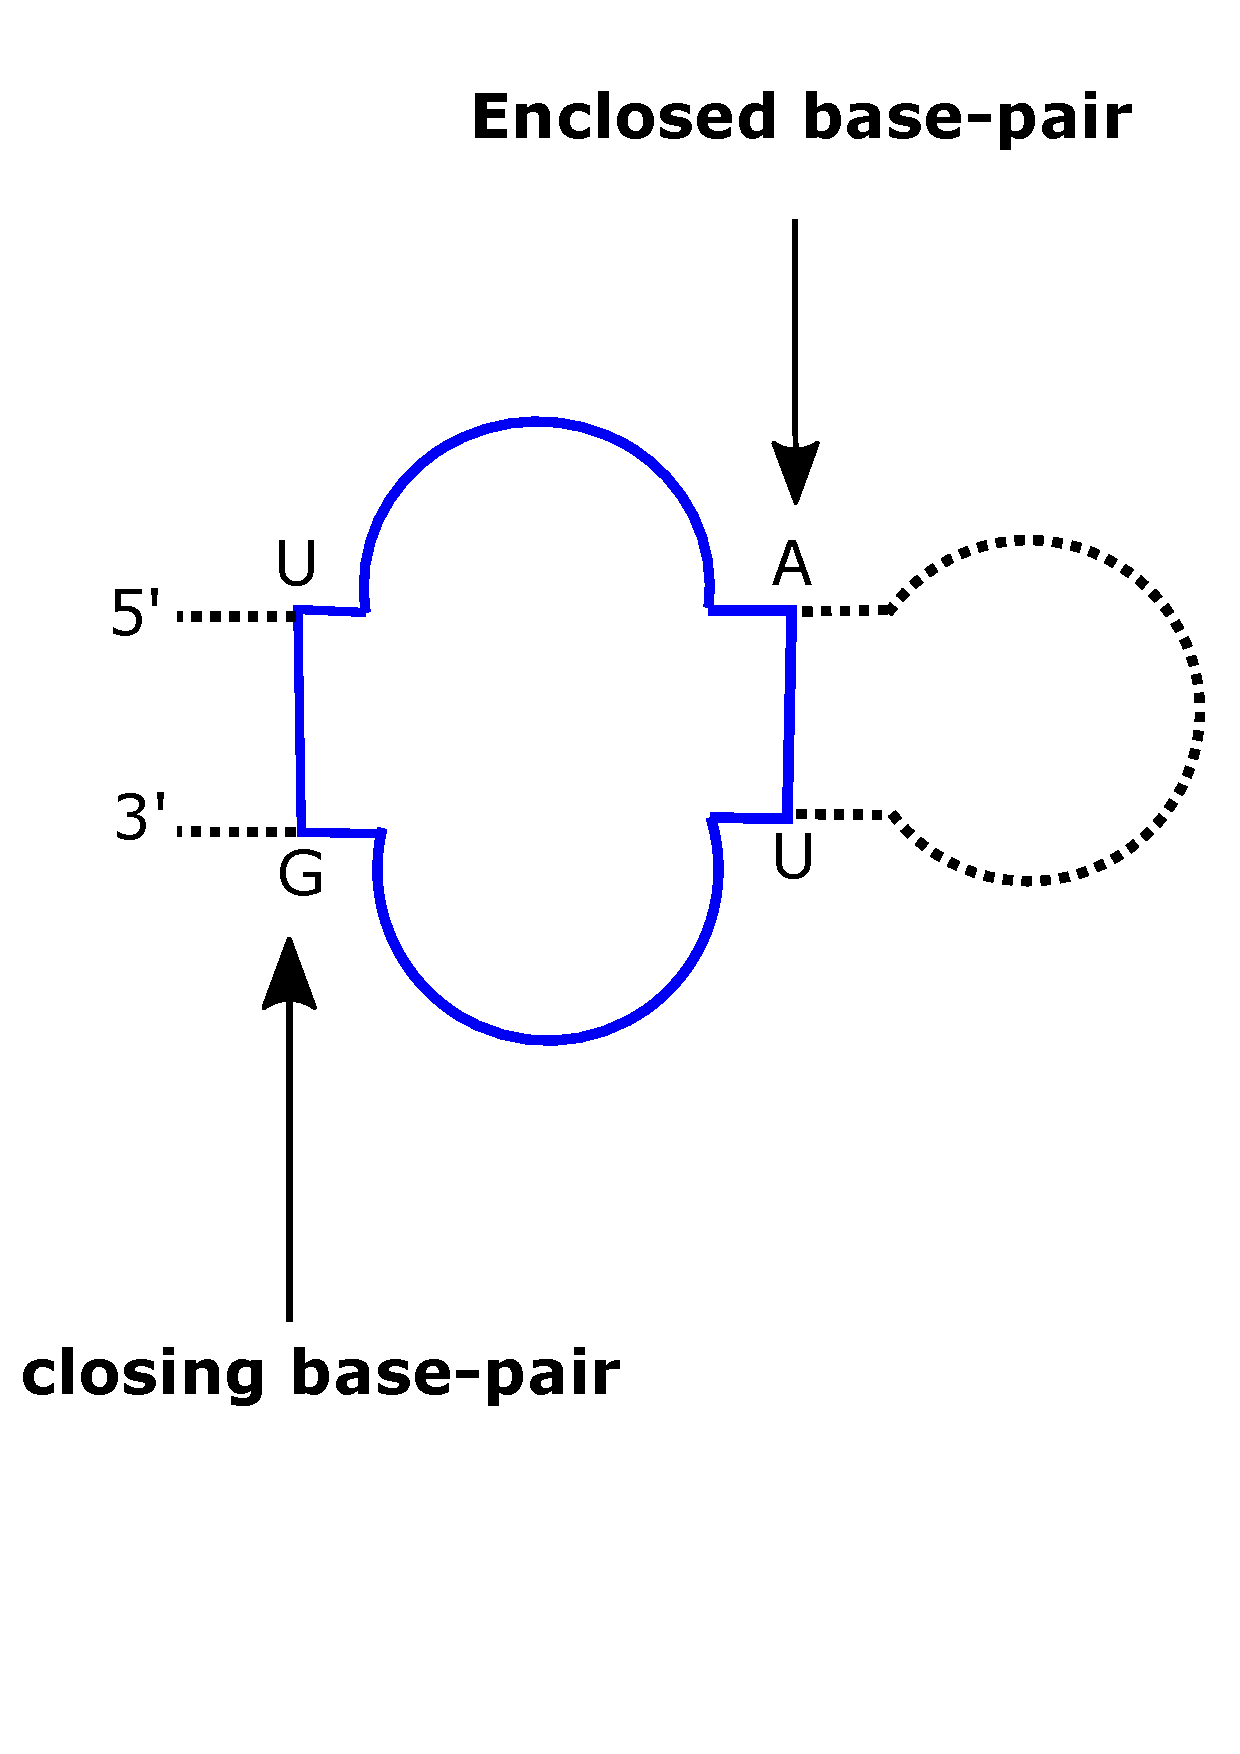
\includegraphics[width=1\linewidth]{../res/images/interior.pdf}
	An example of closing and enclosed base-pairs of an interior loop.
	}	
	
	\begin{enumerate}
		\item Interior loop: a loop with degree $d=2$ i.e $|\mathcal{L}_p|=2$ and $\mathcal{L}_u \subset \{1,2,\dots L\}\cup \emptyset$.
		\item Stacking pair: an interior loop of length $l=0$ i.e. $|\mathcal{L}_p|=2$ and $\mathcal{L}_u = \emptyset$.
		\item Hairpin Loop: Any loop of degree $d=1$ and length $l \geq 3$.  i.e $|\mathcal{L}_p|=1$ and  $\mathcal{L}_u \neq \emptyset$.
		\item Bulge loop: a special case of interior loop in which there are unpaired bases only on one side. i.e  $\mathcal{L}_p=\{(i_1,j_1), (i_2, j_2)\}$ with $i_1 \neq i_2, j_1\neq j_2$ one of the following assumption holds: 
		\begin{itemize}
			\item If $\exists i'\in \mathcal{L}_u \colon i_1<i'<j_2 \Rightarrow \nexists k'\in \mathcal{L}_u \colon i_2<k'<j_2$ 
			\item If $\exists k'\in \mathcal{L}_u \colon i_2<k'<j_2 \Rightarrow \nexists i'\in \mathcal{L}_u \colon i_1<i'<j_1$ 
		\end{itemize}
		\item Multi-loop: Any loop with degree $d>2$ i.e.  $|\mathcal{L}i_p| \geq 3$  and $\mathcal{L}_u \neq \emptyset$.
		\item Exterior loop: a loop in which all the positions are not interior of any pair i.e. $\mathcal{L}_p=\emptyset$ and $\mathcal{L}_u \neq \emptyset$.
	\end{enumerate}
\end{mydef}

\begin{figure}[H]
	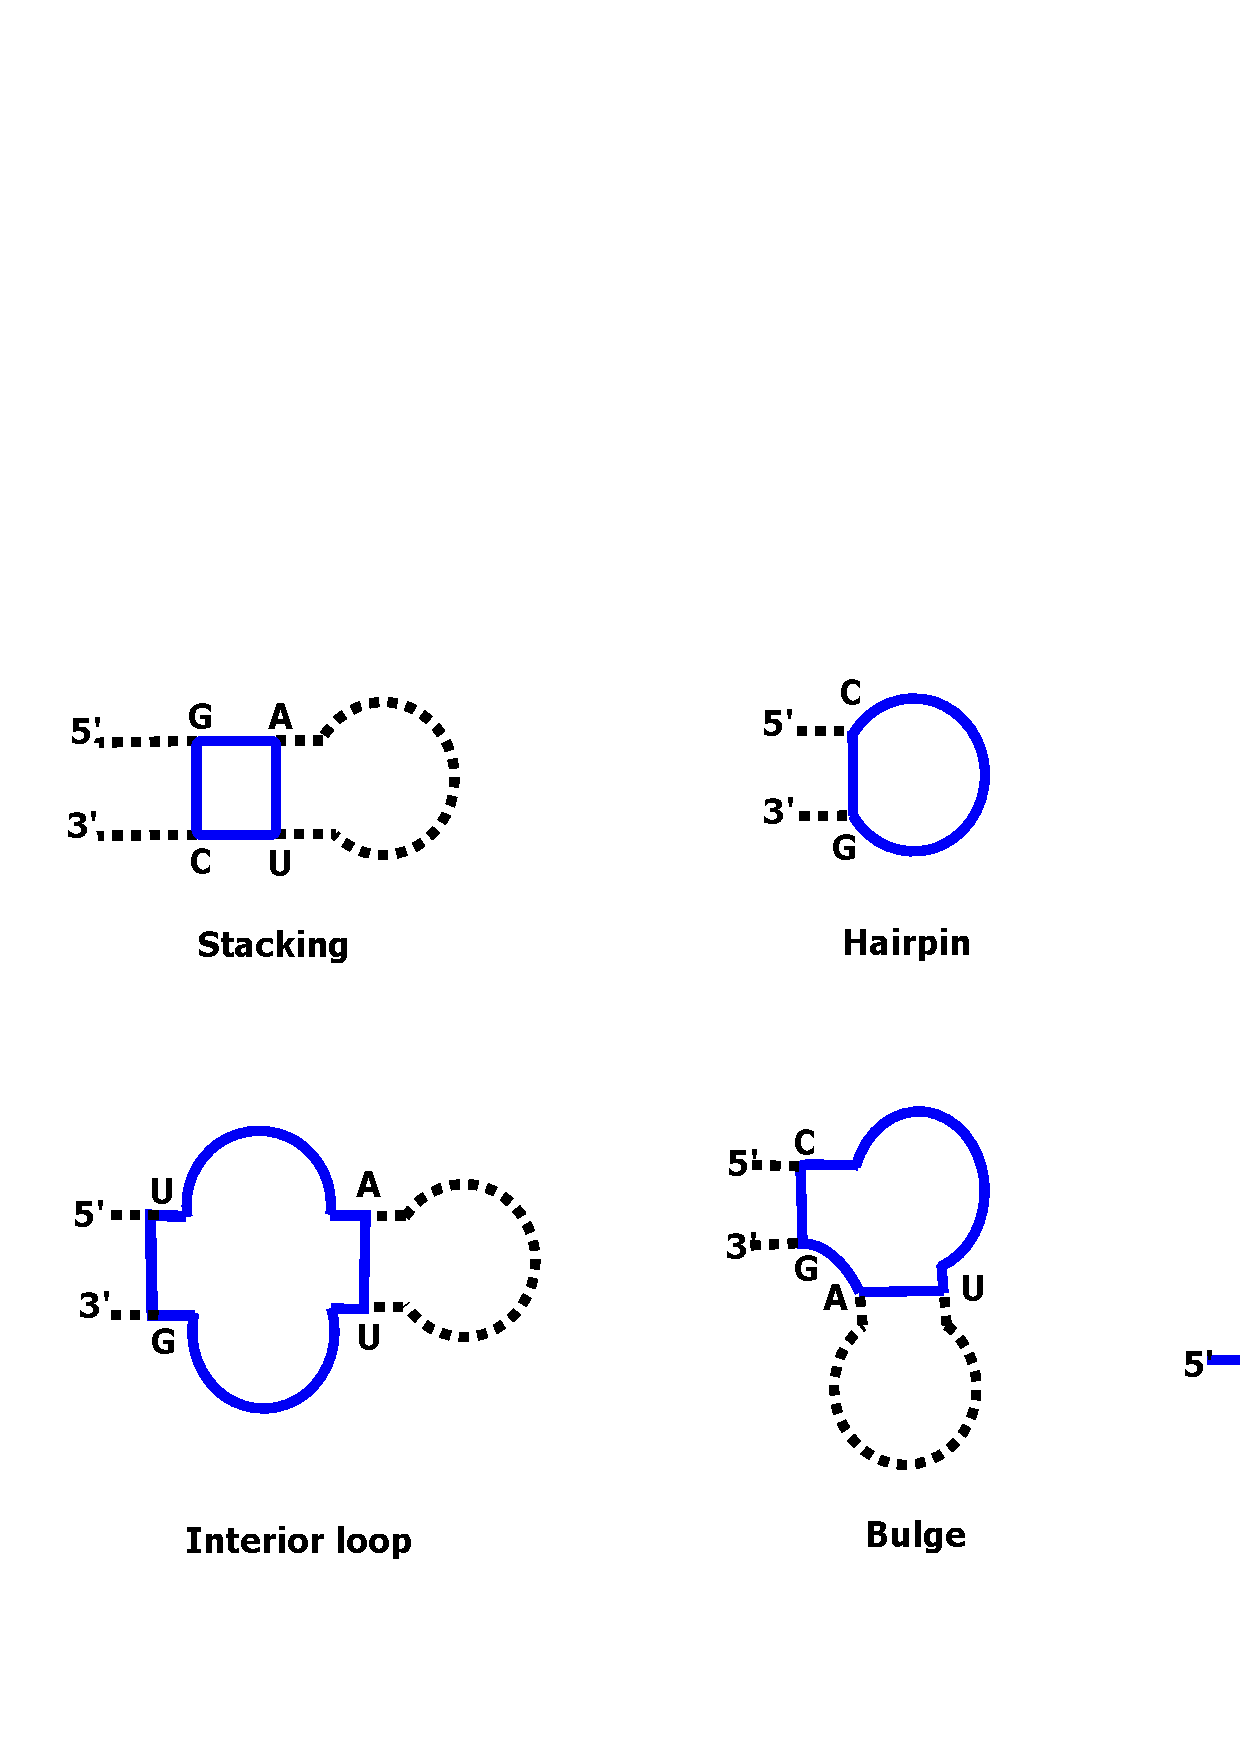
\includegraphics[width=1.0 \linewidth]{../res/images/loops.pdf}
	\caption{\textbf{\ac{RNA} secondary structure loop decomposition}. Each loop is highlighted in blue.}\label{fig:loops}
\end{figure}

\begin{mydef}[Free energy of an \ac{RNA} secondary structure]
	\label{def:free_energy}
	Given the loop set $\mathbb{L}_{\phi, \mathcal{S}}$, the free energy \(\Delta G\) of $\mathcal{S}$ defines its thermodynamic stability. \(\Delta G\) is the free energy difference with respect to the completely unfolded state \cite{tinoco_estimation_1971}. \(\Delta G (\mathcal{S}, \phi)\) is computed using the additivity principle \cite{dill97_addit_princ_bioch}, by summing up the energies of its constituent loops. The free energy \(\Delta G\) is then defined as
	\begin{equation}
	\Delta G(\mathcal{S}, \phi) = \sum_{\mathcal{L}\in \mathbb{L}_{\mathcal{S}, \phi}}{ \Delta G(\mathcal{L}) }.
	\end{equation}
	Many models allow for computing the free energies of those constituent loops, but the dominant is the nearest-neighbor loop energy model \cite{turner09_nndb}. This model associates tabulated free energy values to loop types and nucleotide compositions; the Turner2004 \cite{mathews2004incorporating} is one of the most widely used parameter sets. 
	
	The free energy of each given loop $\mathcal{L}$ is expressed as
	\begin{equation}\label{eq:gibbs}
	\Delta G (\mathcal{L}) = \Delta H - T \Delta S \leq 0
	\end{equation}
	where $\Delta H$ is the (pressure- and volume-dependent) enthalpy change, $T$ the absolute temperature and $\Delta S$ the entropy change. 
	The dominant stabilizing effect is attributed to consecutive base-pairs (The stacking loops), whereas long unpaired regions enclosed between base-pairs have destabilizing effects \cite{fresco_molecular_1960, hofacker_rna_2006}. As a simplified example, the destabilizing free energy contribution $\Delta G(\mathcal{L}_m)$ of a multiloop $\mathcal{L}_m$  as seen in \autoref{fig:loops}C is modelled as
	\begin{equation}\label{eq:multi}
	\Delta G(\mathcal{L}_m) = \Delta G_\mathrm{init} + b \Delta G_\mathrm{branch} + u \Delta G_\mathrm{unpaired}
	\end{equation}
	where $b$ is the number of all surrounding base-pairs and $u$ the number of base-pairs \parencite{dirks_partition_2003}.
\end{mydef}

In addition to the definitions mentioned above, we have various properties of an \ac{RNA} sequence such as structural diversity, positional entropy, structures with maximal expected accuracy, or the density of states. An extensive summary of all possible properties and the history of algorithms is reviewed by Lorenz \cite{lorenz2016predicting}.

The structure decomposition and the tabulated energy parameter sets allow an efficient dynamic programming algorithm to determine a sequence's secondary structure in the entire structure space. Several programs implementing algorithms will enable the computation of these properties efficiently. The thesis gives a literature review of such tools in \autoref{ch:folding}.
\subsection{Thermodynamic definitions}
\label{subsec:thermodynamic_definitions}
A common way to computationally address the \ac{RNA} folding problem is to consider a dynamic system of structures ( the states of the system). Given enough time, a sequence $\phi$ will form every possible structure $\Sigma_{\phi}$. For each structure $\mathcal{S} \in \Sigma_{\phi}$,  there is a probability of observing it at a given time. This subsection defines \ac{RNA} folding thermodynamic properties such as structural ensemble, partition function, Boltzmann probability of a structure $\mathcal{S}$, and the others that derive from them, the base-pair probability and the most probable secondary structure. 

The folding tools such as \texttt{RNAfold}, \texttt{LinearFold} used in this thesis use the same thermodynamic definitions. However, some computational folding methods do not rely on a thermodynamic model. For example,  \autoref{ch:folding} presents a literature review of such tools. 

\begin{mydef}[Structure Ensemble]
	\label{def:structure_ensemble}
	For a given \ac{RNA} sequence $\phi$,  the set of all pseudoknot-free secondary structures with their corresponding energies is called the structure ensemble $\Sigma_{\phi}$ of $\phi$ or Boltzmann ensemble.  We write
	
	$$
	\Sigma_{\phi} = \{ \mathcal{S} | \mathcal{S} \text{ is a secondary structure of $\phi$}\}.
	$$
	
	According to the nearest neighbor energy model, all possible secondary structures of a given \ac{RNA} sequence do not have the same energy. Since each structure has a unique decomposition, each structure has its own energy but different structures can have the same energy.
\end{mydef}
\begin{mydef}[Partition function of \ac{RNA}]
	\label{def:partition_function}
	
	Given the free energy change $\Delta G(\mathcal{S})$ of a structure $\mathcal{S}$, the partition function $Z(\Sigma_{\phi})$ is defined on the Boltzmann ensemble (or structure ensemble) of all possible structures of a given sequence $\phi$ and we write 
	
	\begin{equation}
	Z(\Sigma_{\phi}) = \sum_{\mathcal{S} \in \Sigma_{\phi} }{\exp(-\beta \Delta G(\mathcal{S}, \phi))}
	\end{equation}
	where, $\beta = (RT)^{-1}$ with $R$ the ideal gas constant, and $T$ the temperature.
	
\end{mydef}
\begin{mydef}[Secondary structure probability]
	\label{def:structure_probability}
	How probable is an \ac{RNA} secondary structure $\mathcal{S} \in \Sigma_{\phi}$ for the sequence $\phi$? Given the free energy change $\Delta G(\mathcal{S})$ of a structure $\mathcal{S}$, the boltzmann distribution describes the structure's probability at constant temperature $T$ among all other possible structure of the same sequence $\phi$.
	The probability $p(\mathcal{S}| \phi)$ depends on the free energy $\Delta G(\mathcal{S})$, the lower the more probable. We write
	
	\begin{equation}
	p(\mathcal{S}| \phi)= \frac{\exp(-\beta \Delta G(\mathcal{S}, \phi))}{Z}
	\end{equation}
	where, $Z$ is the partition function and $\beta = (RT)^{-1}$ the thermal constant. 
	
\end{mydef}

\begin{mydef}[\ac{MFE} secondary structure]
	\label{def:mfe}
	
	To predict biologically relevant structures, most computational methods search for structures that minimize the free energy. For a given sequence $\phi$, let~\(\Sigma_{\phi}\) be the secondary structure ensemble of~\(\phi\). The minimum free energy structure $\mathcal{S}_{MFE}$ is the structure with the lowest probability $p(\mathcal{S}|\phi)$ i.e. the  most stable conformation in the thermodynamic equilibrium. We write
	
	\begin{equation}
	\mathcal{S}^{MFE}(\phi) = \arg \min_{\mathcal{S} \in \Sigma_{\phi}} \Delta G(\mathcal{S}, \phi).
	\end{equation}
	
\end{mydef}

\begin{mydef}[Base-pair probability]
	\label{def:bp_probability}
	
	Let $\phi=(\phi_i)_{1\leq i \leq L} $ be an \ac{RNA} sequence. The base-pair probability matrix $\mathbf{P}(\phi)$ quantifies the equilibrium structural features of the ensemble $\Sigma_{\phi}$, with entries $P_{i,j}(\phi) \in [ 0,1]$ defines as 
	
	\begin{equation}
	P_{i,j}(\phi) = \sum_{\mathcal{S} \in \Sigma_{\phi}}{p(\mathcal{S}|\phi)S_{i,j}(\mathcal{S})}.
	\end{equation} 
	
	$P_{i,j}(\phi)$ corresponds to the probability that base-pair $i.j$ forms at the equilibrium. 
	\(\mathbf{S}(\mathcal{S})\) is the structure matrix with entries \(S_{i,j} \in  \{ 0, 1\}\). If the structure \(\mathcal{S}\) contains pair~ $(i ,j)$, then \(S_{i,j}(\mathcal{S}) = 1\)~otherwise \(S_{i,j}(\mathcal{S}) = 0\).
	
	The base-pair probabilities enable then a new view at the structure ensemble. \autoref{fig:bpp} shows an example of \ac{MFE} structure and the base-pair probability dot plot \footnote{computed using \texttt{RNAfold -p}} of a \ac{tRNA}. A square at row $i$ and column $j$ indicates a base-pair. The area of a square in the upper right half of the matrix is proportional to the base-pair probability $(i, j)$ within the equilibrium ensemble. The lower left half shows all pairs belonging to the \ac{MFE} structure. While the \ac{MFE} consists of hairpins, bulge and stacking, several different loops are visualized in the pair probabilities, which leads to several local minima with different shapes.
\end{mydef}
\begin{figure}[t!]
	\includegraphics[width=1.0 \linewidth]{../res/images/trna_bpp.pdf}
	\caption{\textbf{Base-pair probability matrix} of a \ac{tRNA} sequence computed using \texttt{RNAfold 2.4.13}. The \ac{MFE} structure is depicted on the left and the sequence on top. The frequency of the \ac{MFE} structure in the structural ensemble $\Sigma_{\phi}$ is $0.116$. The dot plot on the right shows the pair probabilities within the equilibrium ensemble as ($72\times72$)-matrix and is an excellent way to visualize structural alternatives.  } \label{fig:bpp}
\end{figure}

The definitions mentioned above provide us with a necessary framework enabling us to compute the \ac{MFE} secondary structure within the equilibrium ensemble $\Sigma_{\phi}$. Several implementations of these definitions have been suggested \cite{lorenz11_vienn_packag, reuter2010rnastructure, zadeh2011nupack}, and they are available as an \ac{API}. In the context of this work, we are not only interested in the \ac{MFE} structure but, instead, we use some features of the existing computer libraries (e.g. the computation of the structure free energy) to predict an ensemble structure. The following section introduces some metrics used in this dissertation to compare \ac{RNA} secondary structures and, eventually,  the structure predictions produced by different tools. 
\subsection{Structural distance definitions }
\label{subsec:distance_definitions}
The validation of the results obtained in this thesis is purely empirical. We achieved this goal by comparing the predicted and expected structures for the folding tools. We use the \ac{PPV} and the sensitivity's statistical properties for the benchmark results presented in  \autoref{ch:rafft}. For the inverse folding tools, we compare the \ac{MFE} structure of the designed sequence to the target structure. For that end, a rigorous definition of a measure of similarities between two structures is needed. This subsection defines the different similarity measurements used throughout this work. In addition, it defines the objective functions used in our inverse folding presented in  \autoref{ch:arnaque}. 

\begin{mydef}[The \ac{PPV}]
	\label{def:ppv}
	It measures the fraction of correct base-pairs in the predicted structure and it is defined as
	\begin{equation}
	PPV = \frac{TP}{TP + FP}
	\end{equation}
where TP and FP stand respectively for the number of correctly predicted base-pairs (true positives), and the number of wrongly predicted base-pairs (false positives). 
	
\end{mydef}

\begin{mydef}[Sensitivity]
	\label{def:sensitivity}
	It measures the fraction of base-pairs in the accepted structure that are predicted. We write
	\begin{equation}
	\text{Sensitivity} = \frac{TP}{TP+FN}
	\end{equation}
	where $FN$ stands for the number of base-pairs not detected (false
	negatives).
\end{mydef}
\begin{mydef}[Base-pair distance]
	\label{def:bp_distance}
	Let $\sigma_1$ and $\sigma_2$ be two secondary structures in their string representation.  The base-pair distance between $\sigma_1$ and $\sigma_2$ is defined as
	\begin{equation}
	d_{bp}(\sigma_1, \sigma_2 )= \sum_{i,j} A_{i,j}[\sigma_1] + A_{i,j}[\sigma_2] + 2\times A_{i,j}[\sigma_1] A_{i,j}[\sigma_2],
	\end{equation}
	where, 
	$$
	A_{i,j}[\sigma] =
	\begin{cases}
	1 & \text{if $(i,j)$ is a base-pair in $\sigma$ } \\
	0 & \text{otherwise}.
	\end{cases}
	$$
\end{mydef}

\begin{mydef}[Hamming distance]
	\label{def:hamming_distance}
	Let $\sigma_1$ and $\sigma_2$ be two secondary structures in their string representation. We define the hamming distance between $\sigma_1$ and $\sigma_2$, $d_h(\sigma_1, \sigma_2)$, to be the number of positions where $\sigma_1$ and $\sigma_2$ differ.  We write 
	
	\begin{equation}
	\label{eq:hamming}
	d_h(\sigma_1, \sigma_2) = \sum_{i=1}^{L}{S(\sigma_1^i, \sigma_2^i)}
	\end{equation}
	where, 
	$$
	S(\sigma_1^i, \sigma_2^j) =
	\begin{cases}
	1 & \text{if $\sigma_1^i \neq \sigma_2^j)$ } \\
	0 & \text{otherwise}.
	\end{cases}
	$$
\end{mydef}

\begin{mydef}[\ac{ED}\cite{zadeh2011nucleic}]
	\label{def:ed}
	Given an \ac{RNA} sequence $\phi$ of length $L$, the ensemble defect $\mathcal{D}_E$ is the expected base-pair distance between a target structure $\mathcal{S}^*$  and a random structure generated with respect to the Boltzmann probability distribution. It is defined as 
	\begin{equation}
	\label{ed}
	\begin{split}
	\mathcal{D}_E(\phi, \mathcal{S}^*) 
	&= \sum_{\mathcal{S} \in \Sigma_{\phi}}{p(\mathcal{S}|\phi)d_{bp}(\mathcal{S},\mathcal{S}^*)}\\
	&= L - \sum_{1<i,j<L} P_{i,j}(\phi)S_{i,j}(\mathcal{S}^*)
	\end{split}
	\end{equation}
where~\(P_{i,j}\)~is the base-pair probability matrix entrances, $d_{bp} ((\mathcal{S},\mathcal{S}^*))$ is the base-pair distance between two structures, and \(\mathbf{S}(\mathcal{S})\) is the structure matrix with entries \(S_{i,j} \in  \{ 0, 1\}\). If the structure \(\mathcal{S}\) contains pair~ $(i ,j)$, then \(S_{i,j}(\mathcal{S}) = 1\)~otherwise \(S_{i,j}(\mathcal{S}) = 0\).
\end{mydef}

\begin{mydef}[\ac{NED}]
	\label{def:ned}
	the difference between
	the energy of a given sequence~\(\phi\)~evaluated to fold into a target structure $\mathcal{S}^*$ and the minimum free energy of the sequence in its structural ensemble~\(\Sigma_{\phi}\).~ The value is normalized over all the sequences in a given population $P$.  We write
	
	
	\begin{equation}
	\label{ned}
	\mathcal{N}_E (\phi, \mathcal{S}^*) = [1-\Delta \hat{E}(\mathcal{S}^*,\phi)]^q \text{   } \forall q>1
	\end{equation}
	where,
	\begin{equation}
	\Delta \hat{E}(\mathcal{S}^*, \phi) = \frac{\Delta E(\mathcal{S}^*, \phi) }{\sum_{s \in P}{\Delta E(\mathcal{S}^*, s)}}
	\end{equation}
	and,
	\begin{equation}
	\Delta E(\mathcal{S}^*,\phi) = \Delta G(\mathcal{S}^*, \phi) - \arg \min_{\mathcal{S} \in \Sigma_{\phi\\
	}} \Delta G(\mathcal{S}, \phi).
	\end{equation}
	
\end{mydef}

Among the definitions mentioned above, \autoref{def:ppv} and \autoref{def:sensitivity} are used in \autoref{ch:rafft} for the benchmark comparison. Whereas, definitions \autoref{def:bp_distance}, \autoref{def:hamming_distance}, \autoref{def:ed}, \autoref{def:ned} are used in \autoref{ch:arnaque} for both objective function and benchmark purposes. The following section provides a formal definition of the fitness landscape and some of its properties. It will mostly use \autoref{def:hamming_distance} for both structure and sequence comparison. 

\subsection{\ac{RNA} folding map properties}
\label{subsec:rnamap_properties}
This work considers \ac{RNA} molecule folding and inverse folding optimisation problems. In both cases, It is fundamental to define the fitness landscape notion. This subsection provides the formal definitions of the fitness landscape and examples related to the folding and inverse problem. Some properties such as neutrality, mutation mode or move operator are also provided. The size of the \ac{RNA} structural ensemble has been analytically computed through tools developed by Stein and Waterman \cite{stein1979some}, and it yields an upper bound of~\(S_L\approx1.48\times L^{-\frac{3}{2}}1.85^L\) structure vis-a-vis~\(4^L\) sequences. Compared to the total number of sequences, the number of structures is much smaller, which means there is a high possibility that many sequences fold into the same \ac{MFE} secondary structure. In case that happens, we call the set of those sequences a neutral set. The fraction of such sequences defines the neutrality of a fitness landscape.


\begin{mydef}[Fitness landscape]
	\label{def:fitness_landscape}
	A fitness landscape $\mathfrak{L}$ results from the combination of three elements: a set of configurations $\mathcal{V}$, a cost or fitness function $f$, and a \textit{move} operator $\psi$ that induces a topology on the set of configurations. We write: 
	
	\begin{equation}
	\mathfrak{L} = (\mathcal{G}_f, f, \psi)
	\end{equation}
where $\mathcal{G}_f$  is the the landscape underlying the hypergraph whose vertices are the elements from $\mathcal{V}$ labelled with values given by $f$, and whose edges are specified by the move operator $\psi$.
	
The fitness function $f$ assigns to each configuration $v\in \mathcal{V}$ a real value taken from an interval $ \mathbb{I} \subset \mathbb{R}$ as follows: 

$$
f: \mathcal{V} \rightarrow \mathbb{I}.
$$

An example of fitness function in the case of inverse folding is defined in  \autoref{ch:arnaque} (\autoref{sec:objective_function}), which uses the hamming distance $d_h$ and $\mathcal{V}=\left\{ \text{A}, \text{C}, \text{G}, \text{U} \right\}^L$. But in this case, the fitness defined in the structural space $\Sigma_{\phi}$. i.e. we have an intermediate folding function $\Delta G (\mathcal{S}, \phi)$, mapping any sequence $\phi \in \mathcal{V}$ to an \ac{MFE} secondary structure. 

The move (or mutation) operator $\psi$ defines the relationship between the configuration from  $\mathcal{V}$ in the following way: 
$$
\psi \colon \mathcal{V} \rightarrow \mathcal{V}.
$$
\end{mydef}

\begin{mydef}[Mutation mode]
	\label{def:mutation_mode}
	
	Let $\phi, \phi' \in \mathcal{V} = \left\{ \text{A}, \text{C}, \text{G}, \text{U} \right\}^L$, be  two \ac{RNA} sequences. $\phi'$ is said to be an $n$-point mutation of $\phi$ if it differs from $\phi$ at $n$ nucleotides; i.e. $d_h(\phi, \phi')=n$ where $d_h(.,.)$ is the hamming distance on $\left\{ \text{A}, \text{C}, \text{G}, \text{U} \right\}^L$. 
	
	A mutation mode is a random variable $U$ taking values in $\{1,\dots,L\}$. $P(U=n)$ is defined as the probability that, exactly $n$ nucleotides, selected uniformly at random undergo point mutation during a mutation event. $U$ can generally be any probability distribution.
	
\end{mydef}

\begin{mydef}[Neutral set of \ac{RNA} sequences]
	\label{def:neutral_set}
	For a give fitness landscape $\mathfrak{L} = (\mathcal{G}_f, f, \psi)$, with $\mathcal{V} = \left\{ \text{A}, \text{C}, \text{G}, \text{U} \right\}^L$, two \ac{RNA} sequence $\phi_1$ and $\phi_2$  are set to be neutral $\iff f(\phi_1) = f(\phi_2)$. We call a set $\Gamma \subset \mathcal{V}$ of all such \ac{RNA} sequences a neutral set.  In the case of inverse folding, $\phi_1$ and $\phi_2$ are neutral if they share the same \ac{MFE} secondary structure. In contrast, $\phi_1$ and $\phi_2$ have the same free energy in the folding problem context. 
\end{mydef}

\begin{mydef}[Neutral Network]
	\label{def:neutral_net}
	Let $\mathcal{G} (\mathcal{V}, E)$ be a connected graph in which vertices are all in the neutral sequence set $\Gamma$ (i.e. $\mathcal{V} \subset \Gamma$).  $\mathcal{G}$ is said to be a neutral network $\iff \forall e(v_i, v_j) \in E $,  $v_i,v_j$ differ by a single nucleotide (i.e. $d_h(v_i, v_j)=1$).
\end{mydef}

We provided in this subsection a general definition of a fitness landscape with examples related to computational \ac{RNA} folding and inverse folding. Now that we have all the ingredients to computationally study the folding and the inverse folding of \ac{RNA} molecule, we are left with the definition of some computational techniques used in our proposed tools. Our contributions rely on two well-known techniques of algorithms: the \ac{FFT} for the folding mechanism and the \ac{EA} for the inverse folding. An overview of both techniques is provided in the following section.
\subsection{The fast Fourier transform (FFT) and evolutionary algorithm (EA) applied to RNA bioinformatics}
The computational results present in this work rely on two well-known techniques: the \ac{FFT} and \ac{EA}. Both approaches have already been studied and have found many applications, including the computational folding and inverse folding of \ac{ncRNA}. This section gives a short overview of the two concepts. 

A \ac{FFT} is an algorithm that computes the \ac{DFT} of a sequence or its inverse (\ac{IDFT}). Fourier analysis converts a signal from its original domain (often time or space) to a representation in the frequency domain and vice versa. The \ac{DFT} is obtained by decomposing a sequence of values into components of different frequencies. 

More formally, let $\{x_k\} := x_0, \dots, x_{L-1}$ be a sequence of $L$ complex numbers, the \ac{DFT} transforms the sequence $\{x_k\}$ into another sequence of $L$ complex numbers $\{X_k\} := X_0, \dots, X_{L-1}$ defined as

\begin{equation} 
\label{eq:dft}
X_k = \sum_{n=0}^{L-1}{x_n e^{-i2\pi k n /N}}.
\end{equation} 
%Where, $e^{-i2\pi k n /N}$ is the primitive L$th$ root of $1$.

The direct evaluation of \autoref{eq:dft} will require $O(L^2)$ operations because there are $L$ outputs of $X_k$, and each of them requires a sum of $L$ terms. A \ac{FFT} is, therefore, any approach allowing to compute the same results in $O(L \log L)$ operations \cite{johnson2006modified}.

Let $x$ and $y$ be two sequences of length $L$ and let $X$ and $Y$ be their respective \acp{DFT}. The correlation $c_k$ between sequences $x$ and $y$ with the positional lag of $k$ sites is defined as 

\begin{equation} 
\label{eq:correlation}
c_k = \sum_{1<n<L, 1<n+k<L}{x_ny_{n+k}}.
\end{equation} 
It is known that the correlation $c_k$ can be expressed in terms of the \ac{DFT}. We write 
\begin{equation}
\label{eq:conv}
c_k \Leftrightarrow X^*_n \cdot Y_n
\end{equation}
where the asterisk denotes complex conjugation. That means we simply need to compute the \ac{DFT} $X_n$ and $Y_n$. Therefore, we can compute correlations $c_k$ using the \ac{FFT} as follows: \ac{FFT} the two sequences, multiply one resulting transform by the complex conjugate of the other, and inverse transform the product.

Similar to \autoref{eq:dft}, the direct evaluation of $c_k$ requires $O(L^2)$ operations and taking advantage of the \ac{FFT} reduces it to $O(L \log L)$ operations. Several \ac{FFT} algorithms have been implemented to speed up the computation of the \ac{DFT}
but so far, the most commonly used is the Cooley–Tukey algorithm \cite{cooley1965algorithm}. 

The same idea has been applied in the context of \ac{RNA} bioinformatics, where the two sequences of complex numbers can be thought of as two data sets of real numbers encoding the \ac{RNA} sequences information. And the correlation $c_k$ measures the homologous region in the two \ac{RNA} sequences  \cite{katoh02_mafft}. In contrast to Katoh and his collaborators \cite{katoh02_mafft}, we use the \ac{FFT} to rapidly identify the largest stems of an \ac{RNA} sequence. Thanks to the \ac{FFT} which allows us to efficiently predict the fast-folding pathways of \ac{RNA} molecules (See \autoref{ch:rafft}) within a reasonable \ac{CPU} time.

The \ac{EA} is another well-known heuristic approach, especially when dealing with problems in which less information about the fitness landscape is provided or when there is no exact algorithm in polynomial for such problems. The \ac{EA} approach is inspired by evolutionary systems. In the 1950s and the 1960s, several computer scientists already independently studied evolutionary systems with the idea that evolution could be used as an optimization tool for engineering problems \cite{mitchell1998introduction}. The picture in all these systems was to evolve a population of candidate solutions to a given situation, using operators inspired by natural genetic variation and natural selection.

Since the genetic algorithm (or more generally \ac{EA}) was proposed by John Holland \cite{holland1992adaptation} in the early 1970s, it has emerged as a popular search heuristic. It has found application in many disciplines that deal with complex landscape optimization problems, e.g. RNA folding \cite{montaseri2016evolutionary,wiese2005algorithms} and inverse RNA folding \cite{esmaili2015erd, esmaili2014evolutionary, modena_2012}. 

\begin{figure}[t!]
	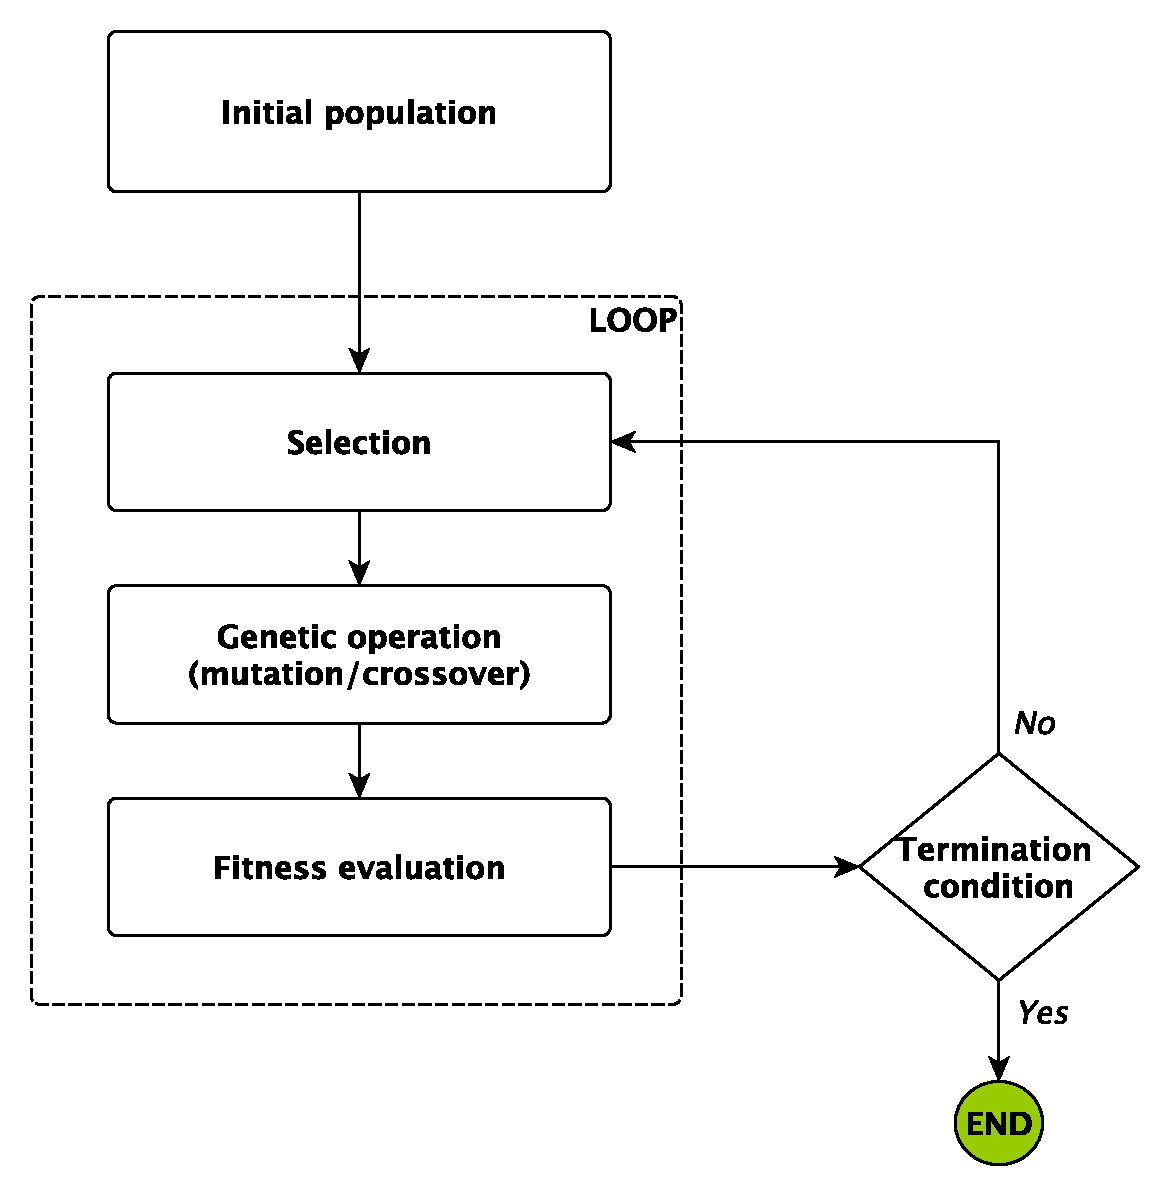
\includegraphics[width=1.0 \linewidth]{../res/images/arnaque/EA_draw.png}
	\caption{\textbf{Evolutionary algorithm flow diagram}. The algorithm initializes a population of candidate solutions and then loops over the three genetic operations until the termination criteria are satisfied. }\label{fig:EA}
\end{figure}

\acp{EA} form a class of heuristic search methods based on a particular
algorithmic framework whose main components are the variation operators
(mutation and recombination or crossover) and the selection operators (parent
selection and survivor selection). The general evolutionary algorithm framework is depicted in \autoref{fig:EA}. In most of the \ac{EA} implementations, the solutions are encoded in the form of genomes (array of elements). The simplest form of \ac{EA} typically involves two types of operators: selection and mutation (single point). 

\begin{itemize}
	\item \textbf{Selection}: the operator consists of selecting solutions in the population for reproduction. The fitter the solution, the more times as likely it is selected to reproduce. This operator often requires a fitness function evaluation.
	\item \textbf{Mutation}: the operator allows generating new solutions in the population. It randomly flips or permutes some element positions in a genome solution.  
	For example, if we encode the solutions in a binary string, the solution $00000100$ might be mutated in its second position to yield $01000100$. Mutation can occur at each bit position in a string with some probability, usually very small (e.g. $0.001$ for a sequence of length $50$).
\end{itemize}

In a more complex configuration, we can have a crossover operator that plays almost the same role as mutation, which generates new solutions in the population. In contrast to the mutation operator,  the crossover randomly chooses a locus and exchanges the subsequence solutions before and after that locus between two solutions to create two offspring solutions. 

In the context of this work, we use the simplest form of \ac{EA}, in which we did not consider a crossover operator. We implement the simplest \ac{EA} framework with a mutation operator adapted to the Inverse folding problem, which results in an alternative computational tool named \texttt{aRNAque} (see \autoref{ch:arnaque})).

This section provided an overview of the two main tools used in this thesis, which are \ac{EA} and \ac{FFT}. The \ac{EA} is implemented in the computational inverse folding tool we propose in \autoref{ch:arnaque}, and the \ac{FFT} in the \ac{RNA} folding tool that will be introduced in \autoref{ch:rafft}. 
\section{Conclusion and outline of the thesis}
\label{sec:ch1_conclusion}
This introductory chapter presents nucleic acids in general and, in particular, a description of \ac{ncRNA} and its chemical, biological, and algorithmic definitions. Those concepts with biological motivations constitute the basis of the thesis. 

We organize the next part of the thesis into fives. The two first s are grouped into a first result part which only concerns \ac{RNA} folding. The second part discusses inverse folding, and similarly to the first part, it contains two s. The last  discusses the presented results and concludes by providing some limitations and possible future research directions. 

In \autoref{pt:folding},  \autoref{ch:folding} provides a brief literature review on the existing computational methods for \ac{RNA} folding. The review focuses on thermodynamic and machine learning methods such as \texttt{RNAfold}, \texttt{LinearFold} and \texttt{Mxfold}. We review some of the limitations of existing tools in  \autoref{ch:folding}, such as the computational time, and in some cases, the predicted thermodynamic structure does not match the native one.  \autoref{ch:rafft} presents our proposed folding tool called \texttt{RAFFT}, which aims at overcoming those limitations. \texttt{RAFFT} implements a novel heuristic to predict \ac{RNA} secondary structure formation pathways that has two components: (i) a folding algorithm and (ii) a kinetic ansatz. This heuristic is inspired by the kinetic partitioning mechanism, by which molecules follow alternative folding pathways to their native structure, some much faster than others. \texttt{RAFFT} starts by generating an ensemble of concurrent folding pathways ending in multiple metastable structures, which contrasts with traditional thermodynamic approaches that find single structures with minimal free energies. When analyzing $50$ predicted folds per sequence, we found near-native predictions for \acp{RNA} of length $\leq 200$ nucleotides, matching the performance of current deep-learning-based structure prediction methods \cite{sato2021rna, zakov2011rich}. \texttt{RAFFT} also acts as a folding kinetic ansatz, which we tested on two \acp{RNA}: the \ac{CFSE} and a classic bi-stable sequence. For the \ac{CFSE}, an ensemble of $68$ distinct structures computed by \texttt{RAFFT} allowed us to produce complete folding kinetic trajectories. In contrast, known methods require evaluating millions of sub-optimal structures to achieve this result. For the second application, only $46$ distinct structures were required to reproduce the kinetics, whereas known methods required a sample of $20,000$ structures. 

Similar to the first part of the result, \autoref{pt:inversefolding} contains two chapters.  \autoref{ch:review_design} will briefly introduce the \ac{RNA} design problem. It distinguishes the positive from the negative \ac{RNA} design problem and reviews the current state of the art computational tools, especially those implementing evolutionary techniques. The existing tools present challenges when benchmarked on recent datasets such as \texttt{Eterna100}. Another limitation is that most existing tools do not consider the pseudoknot patterns in their designing process. In  \autoref{ch:arnaque}, we propose an improved evolutionary algorithm inspired by the Lévy flights. Like a Lévy flight, our tool, \texttt{aRNAque}, implements a Lévy mutation scheme that allows simultaneous search at all scales over the mutational landscape. New mutations often produce nearby sequences (one-point mutations) but occasionally generate mutant sequences far away in genotype space (macro-mutations). In \texttt{aRNAque}, the number of point mutations distribution at every step is taken to follow a Zipf distribution. The Lévy mutation scheme increases the diversity of designed \ac{RNA} sequences and reduces the average number of evaluations of the evolutionary algorithm compared to the local search. The overall performance showed improved empirical results compared to existing tools through intensive benchmarks on both pseudoknot (the \texttt{PseudoBase++} dataset) and pseudoknot-free ( the \texttt{Eterna100} dataset) datasets. 

Finally,  \autoref{ch:conclusion} presents a general conclusion, a discussion on the results obtained and some promising perspectives. It emphasizes the understanding of the Lévy mutation in the context of \ac{RNA} design and the application of our results to evolutionary dynamics. 
